% !TEX root = ../intro-stellar-physics.tex

\section{Hydrostatic equilibrium}
\label{s.hydrostatic-equilibrium}


Consider a fluid at rest in a gravitational field. By a \newterm{fluid}, we mean that the pressure is isotropic\sidenote{Meaning the pressure is the same in all directions.} and directed perpendicular to any given surface. Let's now imagine a small fluid element, as depicted in Fig.~\ref{f.hydrostatic-equilibrium}. The gravitational acceleration is in the direction $-\unitvector{r}$; the fluid element has thickness $\Delta r$ along the direction of the gravitational force and cross-sectional area $\Delta A$.
\begin{marginfigure}
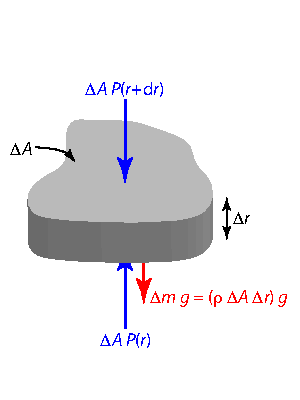
\includegraphics[width=\linewidth]{hydrostatic-equilibrium}
\caption[A fluid element in hydrostatic equilibrium]{A fluid element in hydrostatic equilibrium.
\label{f.hydrostatic-equilibrium}}
\end{marginfigure}

Since our fluid is at rest, the forces must balance. This implies that the pressure only depends on $r$, so that there is no net sideways force on our fluid element. If the fluid has a density (mass per unit volume) $\rho$, then the mass of the fluid element is $\rho\Delta A\Delta r$, and the gravitational force on the fluid element is $-(\rho\Delta A \Delta r) g(r) \unitvector{r}$. This gravitational force is balanced by the \emph{difference} in pressure $P(r)$ between the upper and lower faces of the element.

The pressure force on the upper face is $-\Delta A\times P(r+\Delta r)\unitvector{r}$; on the lower face, $\Delta A\times P(r)\unitvector{r}$. For the element to be in hydrostatic equilibrium the forces along $\unitvector{r}$ must balance,
\[
        \Delta A \left[ -P(r+\Delta r) + P(r) - \Delta r \rho g(r)  \right] = 0.
\]
Dividing by $\Delta r$ and taking the limit $\Delta r \to 0$ gives us the equation of hydrostatic equilibrium:
\begin{equation}\label{e.hydrostatic-equilibrium-g}
        \DD{P}{r} = -\rho g(r).
\end{equation}
This is a differential equation describing how the pressure varies in the star. We don't have enough information yet to solve it, because we haven't specified either the gravity $g(r)$ or the density $\rho$.

\subsection{Constant gravity, incompressible fluid}

Let's try a simple case: an incompressible (density is fixed) fluid in constant gravity. This isn't a good approximation for a star, but it is a good approximation to Earth's oceans: the density of sea water changes by less than 5\% between the surface and ocean floor.

\begin{exercisebox}[Pressure increase in water]
Water is nearly incompressible and has a density $\rho = \val{10^{3}}{\kilo\gram\usk\meter^{-3}}$. Solve eq.~(\ref{e.hydrostatic-equilibrium-g}) to get an equation for the pressure as a function of depth in the ocean. How deep would you need to dive for the pressure to increase by $\val{1}{\unitstyle{atm}} = \val{\sci{1.013}{5}}{\unitstyle{Pa}}$? Does this agree with your experience?
\end{exercisebox}
\marginnote[-3\baselineskip]{The SI unit of pressure is the \textbf{Pascal}: $\val{1}{\unitstyle{Pa}} = \val{1}{\unitstyle{N}\usk\meter^{-2}}$. The mean pressure at terrestrial sea level is $\val{1}{\unitstyle{atm}} = \val{\sci{1.013}{5}}{\unitstyle{Pa}}$. Other common units of pressure are the \textbf{bar} ($\val{1}{\unitstyle{bar}} = \val{10^{5}}{\unitstyle{Pa}}$) and the \textbf{Torr} ($\val{760}{\unitstyle{Torr}} = \val{1}{\unitstyle{atm}}$).}

Let's look at this in a bit more detail.  Suppose we take our fluid layer to be thin, so that $g$ is approximately constant. Then we can write equation~(\ref{e.hydrostatic-equilibrium}) as
\[ \int_{P_{0}}^{P_(z)} \dif P = -g\int_{0}^{z} \rho\,\dif z. \]
Now consider a cylinder of cross-section $\Delta A$ that extends from $0$ to $z$.  The mass of that cylinder is
\[ m(z) = \Delta A\times\int_{0}^{z}\rho \,\dif z.
\]
and its weight is $m(z)g$.
\begin{marginfigure}
\centering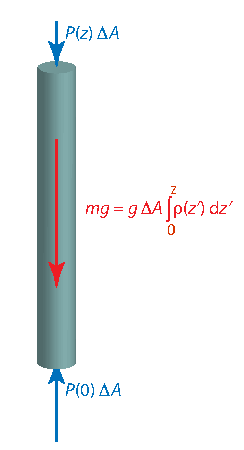
\includegraphics[width=0.8\linewidth]{column}
\caption[The mass of a column of fluid]{
The mass of a column of fluid.
\label{f.column}}
\end{marginfigure}

The difference in pressure between the bottom and top of the cylinder is just
\[ P_{0}-P(z) = g m(z)/\Delta A, \]
that is, the weight per unit area of our column.  Let's apply this to our atmosphere:
if we take the top of our column to infinity and the pressure at the top to zero, then the pressure at the bottom (sea level) is just the weight of a column of atmosphere with a cross-sectional area of $\val{1}{\meter^{2}}$.

\subsection{The isothermal ideal gas}\label{s.ideal-gas}

In general the density $\rho$ depends on the pressure $P$ and temperature $T$ via an \newterm{equation of state}. Let's relax our condition of constant density, but keep gravity and temperature constant and assume the fluid is an ideal gas\sidenote[][\baselineskip]{By \newterm{ideal} gas, we mean that the particles are non-interacting; as a result, the energy of the gas only depends on the kinetic energy of the particles and in particular is independent of the volume.}. For $N$ particles in a volume $V$ at pressure and temperature $P$ and $T$, the ideal gas equation of state is
\begin{equation}\label{e.ideal-gas-eos}
PV = N\kB T
\end{equation}
where $\kB = \val{\sci{1.381}{-23}}{\unitstyle{J}\usk\K^{-1}}$ denotes \newterm{Boltzmann's constant}.

In chemistry, it is convenient to count the number of particles by \newterm{moles}.  One mole of a gas has $\NA = \sci{6.022}{23}$ particles\sidenote{The constant $\NA$ is known as \newterm{Avogadro's number}.}, and the number of moles in a sample is $n = N/\NA$.  If we divide and multiply equation~(\ref{e.ideal-gas-eos}) by $\NA$, then our ideal gas equation becomes
\[ PV = n\left[\NA \kB\right]T \equiv n R T, \]
where $R = \NA\kB = \val{8.314}{\unitstyle{J}\usk\K^{-1}\usk\mol^{-1}}$ is the gas constant. This is perhaps the most familiar form of the ideal gas law---but it is not in a form useful to astronomers.

We astronomers don't care about little beakers of fluid---we have whole stars to model! Put another way, volume isn't a useful quantity since we are working in the middle of a large mass of fluid. Define the \newterm{number density} as the number of particles per volume, $N/V$. The mass of each particle is $\mathcal{A}\times\mb$, where $\mb$ has a mass of one \newterm{atomic mass unit}.\sidenote{$\val{1}{\amu} = \val{\sci{1.661}{-27}}{\kilo\gram}$ is 1/12 of the mass of \val{1}{\mol} of \carbon\ atoms in their ground state} Hence the mass per volume of our fluid is
\[
	\rho = \mathcal{A}\mb \times\frac{N}{V}.
\]
We call $\rho$ the \newterm{mass density}, or density for short. This quantity appears in equation~(\ref{e.hydrostatic-equilibrium-g}).

Starting with eq.~(\ref{e.ideal-gas-eos}), dividing by $V$ and then multiplying and dividing by $\mathcal{A}\mb$ gives
\begin{equation}\label{e.ideal-gas-astro}
 P = \left(\frac{\mathcal{A}\mb N}{V}\right)\frac{\kB}{\mathcal{A}\mb} T \equiv \rho \frac{\kB}{\mathcal{A}\mb} T.
\end{equation}
Equation~(\ref{e.ideal-gas-astro}) is the form most convenient for fluid dynamics, because it is in terms of an intrinsic fluid property---the density $\rho$---rather than in terms of the volume.

\begin{exercisebox}[The isothermal atmosphere]
Let's take a stab at modeling Earth's atmosphere with equation~(\ref{e.hydrostatic-equilibrium-g}). Take Earth's atmosphere to be dry (no water, so we don't have to worry about condensation) and model it as an ideal gas. Also assume the temperature doesn't change with altitude. The average molecular mass of dry air is $\mathcal{A} = 28.97$. Integrate eq.~(\ref{e.hydrostatic-equilibrium-g}) from $z=0$, where $P(z=0)=P_{0}$, to a height $z$. Show that the solution is $P(z) = P_{0}e^{-z/H_{P}}$, where $H_{P}$
is the \newterm{pressure scale height}---the height over which the pressure decreases by a factor $1/e$. Evaluate $H_{P}$ for dry air at a temperature of $\val{288}{\K}$ ($\val{15}{^{\circ}\unitstyle{C}}$). Is the answer reasonable, based on your experience? Is the assumption of an isothermal atmosphere a good one? Explain why or why not.
\end{exercisebox}

The mass $\mathcal{A}$ of an atom or nuclei,
\marginnote{We denote an atomic isotope or nuclide as ${^{A}\mathrm{El}}$, where $A$ is the atomic number (total number of neutrons and protons in the nucleus) and $El$ is the element abbreviation (corresponds to number of protons in the nucleus).}
when expressed in atomic mass units, is approximately equal to the atomic number $A$ (Table~\ref{t.gm-mol}). The electron mass is $m_{e} = \val{0.0005485}{\amu}$. Unless we need high accuracy, we can neglect the electron mass and take the mass of an atom or nuclide to be $A\times\mb$.

\begin{margintable}\caption{\label{t.gm-mol}Selected atomic masses}
\centering
\begin{tabular}{l|rrr}
nuclide & $A$ & $\mathcal{A}$ & $(|\mathcal{A}-A|/A)$ (\%)\\
\hline
\neutron & 1 & 1.00865 & 0.865\\
\hydrogen & 1 & 1.00783 & 0.783\\
\helium & 4 & 4.00260 & 0.065\\
\carbon & 12 & 12.00000 & 0.000\\
\oxygen & 16 & 15.99491 & 0.032\\
\silicon & 28 & 27.97693 & 0.082\\
\iron & 56 & 55.93494 & 0.116\\
\end{tabular}
\end{margintable}

\section{Mass density and the mean molecular weight}
\label{s.mean-molecular-weight}

For a mixture with different types of particles, it is useful to introduce the \newterm{mean molecular weight} $\mu$. This is computed by taking the total mass of a sample of particles and dividing by the total number of particles, so that
\begin{equation}\label{e.mean-mol-weight}
\mu = \frac{\rho}{\mb n_{\mathrm{tot}}} = \frac{1}{\mb}\frac{\sum_{i}m_{i}\,n_{i}}{\sum_{i}n_{i}}.
\end{equation}
Some examples may make this clearer. Suppose we star with molecular hydrogen ($\mathrm{H}_{2}$). The mass of a sample of $n$ molecules is $\approx \val{2}{\mb}\times n$, since each molecule has 2 nucleons. The total number of particles in our sample is $n$, so
\[
	\mu(\mathrm{H_{2}}) = \frac{2\mb \times n}{n\mb} = 2.
\]
Now suppose we raise the temperature and dissociate those molecules into individual atoms. For $n$ atoms, the mass is $\val{1}{\amu}\times n$, so $\mu = 1$. It becomes a little trickier when the atoms are ionized. Let's raise the temperature further, so that the gas ionizes into electrons and nuclei (protons). The electrons contribute negligibly to the mass, so if we have $n$ atoms, the mass is still $\val{1}{\amu}\times n$. The total number of particles has \emph{doubled}, however, since for each atom there are now 2 particles (electron and nucleus). The mean molecular weight is therefore
\[
	\mu(\hydrogen + e^{-}) = \frac{n\mb}{2n\mb} = \frac{1}{2}.
\]
In terms of the mean molecular weight, the ideal gas EOS becomes
\begin{equation}\label{e.eos}
P = \rho\left(\frac{\kB}{\mu\mb}\right) T.
\end{equation}

\begin{exercisebox}[Mean molecular weight for ionized helium]
What is $\mu$ for a fully ionized \helium\ gas ($A=4$, with 2 electrons per atom)? 
\end{exercisebox}

\section{The mass distribution}

Now let's look at how gravity varies within a star. Suppose we are at a distance $r$ from the stellar center. Newton discovered that the gravitational force inside a spherical shell vanished. This means that the net gravitational force arising from portions of the star exterior to our position vanishes. The gravitational force depends only on the amount of mass interior to our position. This mass is
\begin{equation}\label{e.mass-continuity}
	m(r) = 4\pi \int_{0}^{r}\rho(r)r^{2}\,\dif r,
\end{equation}
with $\rho$ being the mass density.

Furthermore, the gravitational force from a spherically symmetric mass is identical to that of a point particle of the same mass. Thus, the gravitational force at a radius $r$ from the center is simply
\[ g(r) = \frac{Gm(r)}{r^{2}}. \]
Using this expression for $g$, we can write eq.~(\ref{e.hydrostatic-equilibrium-g}) as
\begin{equation}\label{e.hydrostatic-equilibrium}
        \DD{P}{r} = -\rho \frac{Gm(r)}{r^{2}}.
\end{equation}

\begin{exercisebox}[At the center]
What happens to $m(r)$ and $g(r)$ at the center ($r\to0$)? Before doing any calculation, see if you can argue that $g(r)\to0$ at the center. If this is so, then what is $\dif P/\dif r$ at the center? Assuming that $\rho\to\rho_{c}\approx\mathrm{const.}$ near the center, integrate eq.~(\ref{e.mass-continuity}) over a small radius $\Delta r$ to get $m(\Delta r)$ and hence $g(\Delta r)$. Show explicitly that $g(\Delta r)\to 0$ as $\Delta r\to0$.
\end{exercisebox}

To recap, we now have two differential equations, (\ref{e.mass-continuity}) and (\ref{e.hydrostatic-equilibrium}), that describe the structure of a star. These equations are for the pressure $P(r)$ and density $\rho(r)$ in the star. We can't solve these equations yet, however, because we don't have a relation between $P$ and $\rho$. For example, the ideal gas equation of state relates $P$ and $\rho$ via a temperature $T$, so we need at least an equation for $T(r)$. Before doing that, let's see what we can learn from just these two equations; to proceed, we shall assume a simple form for $\rho(r)$, such as a constant density, and see what we can infer.

\begin{exercisebox}[A star of constant density]
\label{ex.constant-density-star}
Let's suppose that $\rho$ is constant throughout the star. 
In what follows, you should be able to express everything in terms of the star's mass $M$ and radius $R$, along with physical constants such as $G$ and $\kB$.

\begin{enumerate}
\item\label{rhoc} First, find $\rho$ in terms of the total mass $M$ and radius $R$.

\item Next, solve equation~(\ref{e.mass}) to find $m(r)$ in terms of $M$ and $r/R$.

\item\label{Pc} Use this expression for $m(r)$ and your expression for $\rho$ to integrate equation~(\ref{e.hydrostatic-equilibrium}) and to find the pressure at the center, $P_{c} = P(r=0)$.

\item
Now that we have an expression for the central pressure in terms of $M$ and $R$, let's try to understand what it means. Use your result from parts \ref{rhoc} and \ref{Pc}, as well as equation~(\ref{e.eos}) to find the central temperature of the star, in terms of $G$, $M$, $R$, and the mean molecular weight of the gas $\mu$.  Evaluate $T_{c}$ for $M=M_{\odot}$, $R=R_{\odot}$, and $\mu = 0.6$.  Do you get a reasonable result?
\end{enumerate}
\end{exercisebox}

\section{A closer look at hydrostatic equilibrium}
\label{s.closer-look}

What would happen if the star fell out of equilibrium? Suppose we could turn off the pressure. If we did that, the star would implode. To understand how long this would take, let's calculate the amount of time a particle would need to free-fall from the surface to the center.  We can get this from Kepler's law. Start with a circular orbit and deform it while keeping the center at one focus, as shown in Fig.~\ref{f.fall-to-center}.  

The limit of these increasingly eccentric orbits is a fall into the center.  The time is one-half of an orbital period, and the semi-major axis in this limiting case is $a = R/2$:
\[
\tau_{\mathrm{ff}} = \frac{T}{2} = \frac{\pi}{\sqrt{GM}} \left(\frac{R}{2}\right)^{3/2}.
\]
Notice that we again have the combination $\sqrt{R^{3}/M}$.  Let's convert this into an expression involving the mean density $\bar{\rho}$:
\begin{equation}\label{e.tff}
\tau_{\mathrm{ff}} = \left(\frac{3}{32\pi}\right)^{1/2}\left(\frac{1}{G}\frac{4\pi R^{3}}{3M}\right)^{1/2} = \left(\frac{3}{32\pi}\right)^{1/2} \frac{1}{\sqrt{G\bar{\rho}}}.
\end{equation}
The time to collapse is proportional to $1/\sqrt{G\bar{\rho}}$ and depends on the average density of the star. We call $t_{\mathrm{dyn}} \equiv 1/\sqrt{G\bar{\rho}}$ the \newterm{dynamical timescale} of the star.

\begin{marginfigure}
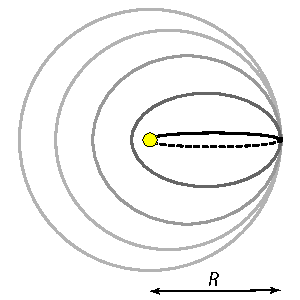
\includegraphics[width=\linewidth]{fall-to-center}
\caption[Fall to center]{\label{f.fall-to-center} Deformation of an orbit until it becomes a fall to the center, denoted by the yellow dot.}
\end{marginfigure}

Let's avoid a collapse by turning the pressure back on.  If part of the star is falling inward, the gas within the star will be compressed, the pressure will rise, and hydrostatic equilibrium will be restored.  How quickly can the star respond? A change is pressure is communicated to the rest of the star by sound waves, which travel at a speed (see Box~\ref{b.sound-speed})
\begin{equation}\label{e.speed-of-sound}
c_{s} = \left(\gamma\frac{P}{\rho}\right)^{1/2}
	= \left(\gamma\frac{\kB T}{\mu\mb}\right)^{1/2}.
\end{equation}
Here $\gamma$ is the adiabatic index: for an ideal monatomic gas, $\gamma = 5/3$.  How long would it take for a sound wave to go a distance $R$?  Using the expression for the average temperature of a constant density sphere from eq.~(\ref{e.mean-T-rho}), we find
\[
	\tau_{\mathrm{sc}} = \frac{R}{c_{s}} = R\left(\frac{3R}{GM}\right)^{1/2}
		= \left(\frac{3}{2\sqrt{\pi}}\right)\frac{1}{\sqrt{G\bar{\rho}}}.
\]
Both the sound-crossing time, $\tau_{\mathrm{sc}}$, and the free-fall time, $\tau_{\mathrm{ff}}$, are approximately equal to the dynamical timescale $1/\sqrt{G\bar{\rho}}$.  This is another way of looking at hydrostatic equilibrium: the star is able to remain in balance because the time for pressure disturbances to propagate, $\tau_{\mathrm{sc}}$, is comparable to the time for large-scale motions of the fluid, $\tau_{\mathrm{ff}}$.

\begin{sidebar}[The sound speed]
\label{b.sound-speed}
Suppose we have a long tube filled with gas at pressure $P(x,t) = P_{0}$, density $\rho(x,t) = \rho_{0}$, and velocity $u(x,t) = U_{0} = 0$. We then tap on one end of the tube; this causes a disturbance to propagate down the tube. Let's look at a small mass of fluid, located between $x$ and $x+\Delta x$; if the cross-sectional area of the tube is $A$, then the mass in this small volume is $\rho A\,\Delta x$.

As a result of the disturbance, the pressure in the tube becomes $P(x,t) = P_{0}+\sigma P_{1}(x,t)$. In this expression, $\sigma$ is a bookkeeping parameter that we'll eventually set to unity. We will expand our equations and keep only terms that are linear in $\sigma$. The fluid will also acquire a velocity $u(x,t) = \sigma u_{1}(x,t)$. This compresses or rarifies the gas: $\rho(x,t) = \rho_{0} + \sigma\rho_{1}(x,t)$.  Because the pressure in the tube is no longer uniform, our small mass will accelerate: 
\begin{eqnarray*}
	\rho A\,\Delta x \ddt{u} &=& A\,\Delta x\,(\rho_{0} + \sigma\rho_{1})\ddt{(0 + \sigma u_{1})}\\
	&\approx& \sigma\left[A\,\Delta x \rho_{0}\ddt{u_{1}}\right] + \mathcal{O}(\sigma^{2}).
\end{eqnarray*}
The corresponding force on our mass is
\[
	A \left[ P(x) - P(x+\Delta x) \right] \approx -\sigma A \left[P_{1}(x+\Delta x)-P_{1}(x)\right];
\]
equating this to the expression---to order $\sigma$---for the acceleration, taking the limit $\Delta x\to 0$, and canceling common factors gives
\begin{equation}\label{e.sound-speed-ut}
	\ddt{u_{1}} = -\frac{1}{\rho_{0}}\ddx{P_{1}}.
\end{equation}
Because of the non-uniform velocity, the volume and hence density of our little mass will also change:
\[
	\ddt{V} = A\left[u(x+\Delta x)-u(x)\right] 
		= \sigma A\,\Delta x\left[\frac{u_{1}(x+\Delta x)-u_{1}(x)}{\Delta x}\right]
\]
or
\begin{equation}\label{e.sound-speed-lnVt}
	\frac{1}{V}\ddt{V} = \sigma \ddx{u_{1}}.
\end{equation}
This change in volume is related to the change in pressure. We are interested in fluctuations that are sufficiently quick that no heat is transferred into or out of our mass. This is an adiabatic process, for which $PV^{\gamma} = \mathrm{const.}$. Here $\gamma$ is called the adiabatic index; for an ideal gas, this is the ratio of specific heats, $\gamma = C_{P}/C_{V}$. (We shall discuss adiabatic processes again more thoroughly in chapter~\ref{ch.main-sequence}.)

As the pressure changes adiabatically from $P_{0}$ to $\sigma P_{1}$, the volume changes as
\[
	\frac{\dif V}{V} = \dif\ln V = -\frac{1}{\gamma}\dif\ln P.
\]
Hence
\begin{equation}\label{e.sound-speed-lnVt-2}
	\ddt{\ln V} = -\frac{1}{\gamma}\ddt{\ln (P_{0} + \sigma P_{1})} \approx 
		-\frac{\sigma}{\gamma P_{0}}\ddt{\ln P_{1}} = \sigma \ddx{u_{1}}.
\end{equation}
The last equality comes from equation (\ref{e.sound-speed-lnVt}).

We therefore have two equations for the perturbed velocity to order $\sigma$:
\begin{eqnarray*}
\ddt{u_{1}} &=& -\frac{1}{\rho_{0}} \ddx{P_{1}}\\
\ddx{u_{1}} &=& -\frac{1}{\gamma P_{0}} \ddt{P_{1}};
\end{eqnarray*}
differentiating the top equation with respect to $x$ and the bottom with respect to $t$, and equating the expressions for $\partial^{2}u_{1}/\partial t\partial x$ gives
\begin{equation}\label{e.sound-speed}
\frac{\partial^{2} P_{1}}{\partial t^{2}} = \left(\frac{\gamma P_{0}}{\rho_{0}}\right)
	\frac{\partial^{2} P_{1}}{\partial x^{2}}.
\end{equation}
This is the equation for a wave: the solutions are $P_{1}(x,t) = P_{1}(x\pm c_{s}t)$, where the sound speed is $c_{s} = \sqrt{\gamma P/\rho}$.
\end{sidebar}

For the sun, $\bar{\rho} = \val{1400}{\kilo\gram\usk\meter^{-3}} = \val{1.4}{\grampercc}$; this is just a bit denser than you.  The dynamical timescale for the sun is about one hour.

\begin{exercisebox}[Sound-crossing time]
The central temperature $T_{c}$ is a measure of the average kinetic energy of a particle at the stellar center. Use the central temperature that you found for the constant density star in exercise~\ref{ex.constant-density-star} and estimate the time that such a particle would take to cross a distance $R$. How does this time compare to the orbital period of a satellite orbiting just outside the stellar surface?
\end{exercisebox}

\section{Virial Equilibrium}
\label{s.virial-equilibrium}

With the assumption that $\rho = \textrm{constant}$, we showed (exercise~\ref{ex.constant-density-star}) that the central temperature and pressure depended on the total mass $M$, total radius $R$, and the gravitational constant $G$ as
\begin{eqnarray}
\label{e.Tc}
T_{c} &=& \frac{1}{2}\left\{\frac{GM}{R}\frac{\mu\mb}{\kB}\right\}\\
\label{e.Pc}
P_{c} &=& \frac{3}{8\pi}\left\{\frac{GM^{2}}{R^{4}}\right\}.
\end{eqnarray}
Here $\mu\mb$ is the average mass of a particle in the plasma\sidenote{%
The constant $\mb$ is defined as $1/12$ the mass of a \carbon\ atom.}.
Our task now is to show that the scalings of $T_{c}$ and $P_{c}$ with $M$ and $R$---the quantities in $\{\,\}$---hold in general for an a star in mechanical equilibrium.

To show this, we are going to employ a form of the \emph{virial theorem}.  Suppose we have a collection of $N$ particles, all moving about and exerting forces on one another.  If we let this system settle down into some kind of bound configuration, then we can add up the kinetic and potential energies of all the particles to get a total kinetic energy $K$ and a total potential energy $\Omega$. The virial theorem asserts that $K$ is proportional to, and comparable in magnitude to, $\Omega$; indeed if the potential between a pair of particles scales as $r^{-1}$, $r$ being the distance between the particles, then $K = -\Omega/2$, as we'll now show.

Let us take the position and momentum of particle $i$ to be $\bvec{r}_{i} = (x_{i},y_{i},z_{i})$ and $\bvec{p}_{i}=(p_{x},p_{y},p_{z})$.  Then the total kinetic energy is
\begin{eqnarray}
\nonumber
	K &=& \frac{1}{2}\sum_{i=1}^{N}\bvec{p}_{i}\vdot\DDt{\bvec{r}_{i}}\\
		&=& \frac{1}{2}\left[\DDt{}\left(\sum_{i=1}^{N}\bvec{p}_{i}\vdot\bvec{r}_{i}\right) - \sum_{i=1}^{N}\bvec{r}_{i}\vdot\DDt{\bvec{p}_{i}}\right].
\label{e.expand-K}
\end{eqnarray}
The quantity $G = \sum_{i}\bvec{p}_{i}\vdot\bvec{r}_{i}$ is called the ``virial'' of the system.  By expressing the force $\bvec{F}_{i} = \dif\bvec{p}_{i}/\dif t$ on particle $i$ as the gradient of a potential $\Omega$, $\bvec{F}_{i} = -\grad_{i}\Omega$, we can rewrite eq.~(\ref{e.expand-K}) as
\begin{equation}\label{e.virial-deriv-1}
	2K = \DDt{G} + \sum_{i=1}^{N}\bvec{r}_{i}\vdot\grad_{i}\Omega.
\end{equation}
So far, we just shuffled and relabeled terms.  The crucial step comes in taking the time-average of the kinetic energy, which we'll denote by $\langle\;\rangle$:
\[	\langle f\,\rangle \equiv \lim_{\tau\to\infty} \frac{1}{\tau}\int_{0}^{\tau}f(t)\,\dif t. \]
Applying this to equation~(\ref{e.virial-deriv-1}) gives
\begin{eqnarray*}
	2\langle K\,\rangle &=&
		 \left\langle\DDt{G}\right\rangle 
		+ \left\langle\sum_{i=1}^{N}\bvec{r}_{i}\vdot\grad_{i}\Omega\right\rangle\\
	&=& \lim_{\tau\to\infty}\left[\int_{0}^{\tau}\,\DDt{G}\,\dif t\right] 
		+ \left\langle\sum_{i=1}^{N}\bvec{r}_{i}\vdot\grad_{i}\Omega\right\rangle\\
	&=& \underbrace{\lim_{\tau\to\infty}\left[\frac{G(\tau)-G(0)}{\tau}\right]}_{\mathrm{I}}
		+ \underbrace{\left\langle\sum_{i=1}^{N}\bvec{r}_{i}\vdot\grad_{i}\Omega\right\rangle}_{\mathrm{II}}
\end{eqnarray*}
Now, if the system is bound and in mechanical equilibrium, then the positions and momenta of all particles are finite: none of the particles can escape, and the system doesn't violently collapse so that momenta are diverging.  Hence both $G(\tau)$ and $G(0)$ are finite numbers, so as $\tau\to\infty$, term I vanishes.

As for term II, we can show that if the potential between pairs of particles depends on $1/r$, where $r$ is the distance between those particles, then term II is just $-\Omega$ (see Box~\ref{b.working-vectors}).  For now, I'll give a rough argument of why this is so:  in a spherically symmetric system, then the potential just depends on the distance $r$ from the origin; and since
\[
	r\dd{}{r} \left(\frac{1}{r}\right) = -\frac{1}{r},
\]
the last term is just $-\Omega$ and our equation is
\begin{equation}\label{e.virial-theorem}
2\langle K\,\rangle + \langle \Omega\rangle = 0.
\end{equation}
This is the virial theorem.

\begin{sidebar}[Working with vectors]
\label{b.working-vectors}
In this sidebar we'll show that the second term in equation~(\ref{e.virial-deriv-1}) is
\begin{equation}\label{e.term-2}
	\sum_{i=1}^{N}\bvec{r}_{i}\vdot\grad_{i}\Omega = -\Omega.
\end{equation}
First, we need an expression for $\Omega$. Suppose we pick a pair of particles, $i$ and $k$.  The potential between this pair is
\[
	-\frac{Gm_{i}m_{k}}{r_{ik}} = -\frac{Gm_{i}m_{k}}{\sqrt{(\bvec{r}_{i}-\bvec{r}_{k})^{2}}}.
\]
Our total potential consists of a sum over the potentials between all $N(N-1)/2$ unique pairs of particles,
\[
	\Omega = -\frac{Gm_{1}m_{2}}{\sqrt{(\bvec{r}_{1}-\bvec{r}_{2})^{2}}} - \ldots 
	-\frac{Gm_{i}m_{k}}{\sqrt{(\bvec{r}_{i}-\bvec{r}_{k})^{2}}} - \dots
\]
When we take the derivative in eq.~(\ref{e.term-2}), we apply $\bvec{r}_{i}\vdot\grad_{i}$ to each term in the potential.  For the term with the pair $i$, $k$, this will give
\begin{eqnarray*}
	\lefteqn{\sum_{i=1}^{N}\bvec{r}_{i}\vdot\grad_{i}\left(-\frac{Gm_{i}m_{k}}{\sqrt{(\bvec{r}_{i}-\bvec{r}_{k})^{2}}}\right)} \\
	&=& -Gm_{i}m_{k}\left[\bvec{r}_{i}\vdot\grad_{i}\left(\frac{1}{\sqrt{(\bvec{r}_{i}-\bvec{r}_{k})^{2}}}\right) + \bvec{r}_{k}\vdot\grad_{k}\left(\frac{1}{\sqrt{(\bvec{r}_{i}-\bvec{r}_{k})^{2}}}\right)\right].
\end{eqnarray*}
Since many of you aren't yet comfortable with vector expressions, we'll do this in detail for the $x$-component:
\begin{eqnarray*}
	\lefteqn{\left[\bvec{r}_{i}\vdot\grad_{i}\left(\frac{1}{\sqrt{(\bvec{r}_{i}-\bvec{r}_{k})^{2}}}\right) + \bvec{r}_{k}\vdot\grad_{k}\left(\frac{1}{\sqrt{(\bvec{r}_{i}-\bvec{r}_{k})^{2}}}\right)\right]_{x}}\\
	&=& x_{i}\dd{}{x_{i}}\left(\frac{1}{\sqrt{(\bvec{r}_{i}-\bvec{r}_{k})^{2}}}\right)
		+ x_{k}\dd{}{x_{k}}\left(\frac{1}{\sqrt{(\bvec{r}_{i}-\bvec{r}_{k})^{2}}}\right) \\
		&=& -\frac{x_{i}(x_{i}-x_{k})}{(\bvec{r}_{i}-\bvec{r}_{k})^{3/2}}
		+ \frac{x_{k}(x_{i}-x_{k})}{(\bvec{r}_{i}-\bvec{r}_{k})^{3/2}}\\
		&=& -\frac{(x_{i}-x_{k})^{2}}{(\bvec{r}_{i}-\bvec{r}_{k})^{3/2}}
\end{eqnarray*}
The $y$- and $z$-components are similar, giving
\begin{eqnarray*}
	\sum_{i=1}^{N}\bvec{r}_{i}\vdot\grad_{i}\left(-\frac{Gm_{i}m_{k}}{\sqrt{(\bvec{r}_{i}-\bvec{r}_{k})^{2}}}\right) &=& Gm_{i}m_{k}
	\frac{(\bvec{r}_{i}-\bvec{r}_{k})^{2}}{(\bvec{r}_{i}-\bvec{r}_{k})^{3/2}}\\
 &=& -\left(-\frac{Gm_{i}m_{k}}{\sqrt{(\bvec{r}_{i}-\bvec{r}_{k})^{2}}}\right).
\end{eqnarray*}
This can be done for every term in the sum, with the final result that
\[
	\sum_{i=1}^{N}\bvec{r}_{i}\vdot\grad_{i}\Omega = -\Omega.
\]
\end{sidebar}

For an ideal monatomic gas in thermal equilibrium, the mean kinetic energy of a particle in the gas is $K = (3/2)\kB T$, and we therefore may define an average temperature
\begin{equation}\label{e.Tbar}
	2 K = 3 N\kB \bar{T} = -\Omega.
\end{equation}
The total number of particles is $N=M/(\mu\mb)$, and so
\begin{equation}\label{e.mean-T}
\bar{T} = -\frac{1}{3}\Omega\frac{\mu\mb}{M\kB}.
\end{equation}
The total potential of the system depends on only three parameters: $G$, $M$, and $R$.  The only way to make a quantity having dimensions of energy is for
\[ \Omega \propto -\frac{GM^{2}}{R}, \]
and so
\[ \bar{T} \propto \frac{GM}{R}\frac{\mu\mb}{\kB}.  \]
By using the ideal gas law, $\bar{P} = \bar{\rho}(\kB/\mu\mb)\bar{T}$, we find
\[ \bar{P} \propto \frac{GM^{2}}{R^{4}}. \]
As a concrete example, let's compute $\Omega$ for a constant density sphere.
If we bring a small amount of mass $\dif m$ from infinity onto a sphere of mass $m$ and radius $r$, then the change in potential is \[ \dif\Omega = -\frac{Gm}{r}\,\dif m. \]
For a constant density, $r = R(m/M)^{1/3}$; upon substituting for $r$ we have
\begin{equation}\label{e.energy-constant-density-sphere}
	\Omega_{\textrm{const.\ den.}} = - \int_{0}^{M}\frac{GM^{1/3} m^{2/3}}{R}\,\dif m = -\frac{3}{5}\frac{GM^{2}}{R}.
\end{equation}
Using this in equation~(\ref{e.mean-T}) gives us the mean temperature, and hence pressure, for a constant density sphere,
\begin{eqnarray}\label{e.mean-T-rho}
\bar{T} &=& \frac{1}{5}\frac{GM}{R}\frac{\mu\mb}{\kB},\\
\label{e.mean-P}
\bar{P} &=& \frac{3}{20\pi}\frac{GM^{2}}{R^{4}}.
\end{eqnarray}
These are comparable to the central values, eqn.~(\ref{e.Tc}) and (\ref{e.Pc}).

\begin{table}
\caption[Masses, radii, and luminosities for selected stellar types]{\label{t.stellar-properties} Masses, radii, and luminosities for selected stellar types. The type---B2, B8, F0, and so forth---indicates what features are present in the star's spectrum and indicates the star's surface effective temperature.}
\begin{tabular}{ld{4.2}d{3.2}d{1.2}d{1.2}d{1.2}d{1.2}d{2.3}}
 & \tabhead{B2} & \tabhead{B8} & \tabhead{F0} & \tabhead{F5} & \tabhead{G5} & \tabhead{M0} & \tabhead{M7}\\ 
\hline
$M/\Msun$ & 9.8 & 3.8 & 1.6 & 1.3 & 0.92 & 0.51 & 0.12\\
$R/\Rsun$ & 5.6 & 3.0 & 1.5 & 1.3 & 0.92 & 0.60 & 0.18\\
$L/\Lsun$ & 5800.0    & 180.0 & 6.5 & 3.2 & 0.79 & 0.08 & 0.003\\
\end{tabular}
\end{table}

\begin{exercisebox}[Applications of virial scalings]\label{ex.stellar-properties}
We can infer a great deal from our simple virial scalings. Table~\ref{t.stellar-properties} provides masses, radii, and luminosities, in units of $\Msun$, $\Rsun$, and $\Lsun$, for stars from type B (hot blue stars) to type M (cool red stars).  
Using the constant density model, compute $\rho/\rho_{\odot}$, $T_{c}/T_{c,\odot}$, and $P_{c}/P_{c,\odot}$. You should find that each quantity depends only on $m=M/\Msun$ and $r=R/\Rsun$. Describe your findings: do $P_{c}/P_{c,\odot}$, $\rho/\rho_{\odot}$, and $T_{c}/T_{c,\odot}$ vary in a similar fashion? If not, how do they change with stellar type?
\end{exercisebox}

\section{Contraction to the main sequence}
\label{s.stellar-contraction}

Stars are born when a cold, dense\sidenote{Dense is a relative term; here we mean $\sim 100$ \emph{atoms} per cubic centimeter} cloud of gas and dust becomes unstable to gravitational collapse. The details of this process is a topic of current research; for our purposes, however, after a period of time a pre-main sequence star forms.  This object is in hydrostatic balance, but with a radius much larger than its main-sequence value.  As you know from the previous discussion, its central temperature will therefore be too low for fusion reactions to be important.  What happens to this object?

The pre-main sequence star is in hydrostatic balance, so it doesn't collapse. But the interior, and hence the surface, is warm, so it radiates energy.  The only source of energy is gravitational, so the pre-main sequence star \emph{must} contract.  How long would this take?  For our sun, the total energy is
\[
	E_{\odot} = K + \Omega = \Omega/2 \approx -\frac{G\Msun^{2}}{\Rsun};
\]
the time to radiate this energy away is
\begin{equation}\label{e.kelvin-helmholtz}
t_{\mathrm{KH}} = \frac{|E_{\odot}|}{\Lsun} \approx \frac{G\Msun^{2}}{\Rsun\Lsun} \approx \val{\sci{3}{7}}{\yr}.
\end{equation}
This timescale is called the \newterm{Kelvin-Helmholtz timescale}.  Since $t_{\mathrm{KM}} \gg t_{\mathrm{dyn}}$ the star is, to an excellent approximation, in hydrostatic equilibrium throughout the whole contraction.

\begin{exercisebox}[Contraction of a constant density protostar]
\label{ex.contraction-constant-density-protostar}
Using the constant-density model (constant here means ``constant throughout the star at any given time'') and the virial relations, give a qualitative sketch for how the pressure, density, temperature, radius, and total energy change with time as the protostar contracts.
\end{exercisebox}

\begin{exercisebox}[The relation between energy and temperature]
\label{ex.gravithermal-specific-heat}
Using the constant density model, derive an expression for the total energy (kinetic plus potential) as a function of central temperature. Plot this relation.  What happens to the central temperature if additional heat is injected into the star?
\end{exercisebox}

\begin{exercisebox}[The oscillation period of a star]
\label{ex.stellar-oscillation-period}
Let's revisit our constant density model from exercise \ref{ex.constant-density-star}. Let's consider a thin outer layer. The pressure on the upper surface vanishes, and the pressure on the bottom is $P(R)$.

\begin{enumerate}
\item\label{ex.math-prelim}
As a mathematical preliminary, suppose we have a function $f(x) = Ax^{\alpha}$ and that we expand about a point $x_{0}$ with $f_{0} = Ax_{0}^{\alpha}$. Show that to lowest order in $\delta x$,
\[
	f(x_{0}+\delta x) \approx f_{0}\left( 1 + \alpha\frac{\delta x}{x} \right).
\]

\item
Write $\dif P/\dif r$ as $\Delta P/\Delta r$, where $\Delta r$ is the thickness of the layer, and then integrate the equation of hydrostatic balance (\ref{e.hydrostatic-equilibrium}) over the surface to show that
\begin{equation}\label{e.shell-pressure-balance}
	4\pi R^{2} P(R) - \frac{GMm}{R^{2}} = 0,
\end{equation}
where $m = 4\pi R^{2}\Delta r \rho$ is the mass of the layer. For the rest of this exercise, we shall take $m$ as fixed.

\item
Now suppose of star expands by a small amount $\delta R$. Use the result of part \ref{ex.math-prelim} to find the new density $\rho'$ in terms of the original density $\rho$ and $\delta R$, to lowest order in $\delta R/R$.

\item
If the contraction is adiabatic, then the new pressure obeys a relation $P' V'^{\gamma} = PV^{\gamma}$ (cf.\ Box \ref{b.sound-speed}). For our shell of mass $m$, show that this implies that $P'\rho'^{-\gamma} = P\rho^{-\gamma}$, and thus find $P'$ in terms of $P$, $\delta R/R$, and $\gamma$, to lowest order in $\delta R/R$.

\item
Insert the expressions for $P'$ and $R'=R+\delta R$ into equation~(\ref{e.shell-pressure-balance}) and cancel any common factors; you should find that the pressure and gravitational forces no longer balance. Express the residual force in terms of $GMm/R^{2}$, $\gamma$ and $\Delta R/R$.

\item
Equate this residual force with the acceleration of the shell, $m\ddot{\delta R}$, and show that the shell oscillates. For $\gamma = 5/3$ (appropriate for an ideal gas), find the period of oscillation in terms of $\rho = 3M/4\pi R^{3}$.
\end{enumerate}
\end{exercisebox}

